\documentclass{report}

\usepackage{graphicx}
\usepackage{amsmath}
\usepackage{physics}

\newcommand{\ve}[1]{\mathbf{#1}}

\begin{document}

We begin by looking at a rod pivoting on a surface under gravity without
slipping. The configuration of this is shown in this diagram:
\newline
\begin{center}
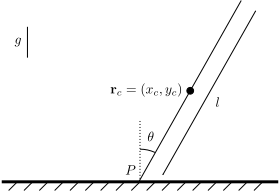
\includegraphics{rod_geometry.pdf}
\end{center}
We use a standard horizontal/vertical $x,y$ coordinate system with the origin
located at the contact point $P$ between the rod and surface. Since the rod is
not slipping the contact point is stationary. We can also say that the centre
of mass position vector in this coordinate system is
\begin{equation*}
  \ve{r}_c
      = (x_c, y_c)
      = \left(\frac{l}{2}\sin\theta, \frac{l}{2}\cos\theta\right)
\end{equation*}
The free forces acting on the rod are the weight $mg$ acting at the centre of
mass and the normal reaction $N$ and friction $F$ (tangential reaction)
acting at the contact point $P$. The free body diagram for the rod is shown
here:
\newline
\begin{center}
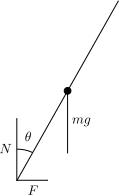
\includegraphics{rod_free_body.pdf}
\end{center}

Newton's third law for the horizontal and vertical forces gives
\begin{align*}
  m\ddot{x}_c &= F \\
  m\ddot{y}_c &= N - mg
\end{align*}
Since $P$ is fixed in an inertial frame we can apply the torque equation
$\dv{L_P}{t} = T_P$ where $L_P$ is the angular momentum of the rod around
point $P$ and $T_P$. For the rod this gives
\begin{equation*}
  \dv{L_P}{t}
  = \dv{(I_P \dot{\theta})}{t}
    = I_P \ddot{\theta}
    = (m\left(\frac{l}{2}\right)^2 + \alpha m l^2) \ddot{\theta}
    = mg \frac{l}{2} \sin{\theta}
\end{equation*}
where the moment of inertia for the rod around its centre of mass is $I_c =
\alpha ml^2$ and we have used the parallel axis theorem to get $I_P$.
Bringing our three differential equations for the rod together we have
\begin{equation}
  \begin{aligned}
    &\ddot{x}_c = \frac{F}{m} \\
    &\ddot{y}_c = \frac{N}{m} - g
            = \frac{N}{m} - \frac{l}{2}\omega^2 \alpha_P \\
    &\ddot{\theta} = \frac{2g}{(1+4\alpha)l} \sin{\theta}
        = \frac{2g}{l\alpha_P} \sin{\theta}
        = \omega^2 \sin{\theta}
  \end{aligned}
  \label{eq:nls_rod}
\end{equation}
where $\alpha_P = (1 + 4\alpha)$ is $4\times$ the inertia coefficient around
$P$ and $\omega^2 = \frac{2g}{l\alpha_P}$.

The forces $F$ and $N$ are the tangential and normal reaction forces at the
rod/surface contact point. As reaction forces their value must be determined
from the constraint that they ensure. In this case the constraint is that the
end of the rod remains in contact with the surface and that the end of the rod
does not slip on the durface. Together these are that the end of the rod is
stationary at $P$. This constrains $x$ and $y$ in terms of $\theta$ since we
have
\begin{equation*}
  x_c = \frac{l}{2}\sin\theta \quad y_c = \frac{l}{2}\cos\theta.
\end{equation*}
Differentiating twice with respect to $t$ we get
\begin{align*}
  \ddot{x}_c &= \frac{l}{2}(\ddot{\theta}\cos\theta - \dot{\theta}^2\sin\theta) \\
  \ddot{y}_c &= -\frac{l}{2}(\ddot{\theta}\sin\theta + \dot{\theta}^2\cos\theta)
\end{align*}
We can then obtain the necessary reaction forces $F$ and $N$
from~\eqref{eq:nls_rod} as
\begin{align*}
  F &= \frac{ml}{2} (\ddot{\theta}\cos\theta - \dot{\theta}^2\sin\theta) \\
  N &= \frac{ml}{2}\omega^2\alpha_P-\frac{ml}{2} (\ddot{\theta}\sin\theta + \dot{\theta}^2\cos\theta).
\end{align*}
The rod can only remain resting on the floor if the normal reaction force $N$
needed is positive so a consistency condition is that $N \ge 0$. This gives
that
\begin{equation*}
  \omega^2\alpha_P - (\ddot{\theta}\sin\theta + \dot{\theta}^2\cos\theta)
  = \omega^2\alpha_P - (\omega^2\sin^2\theta + \dot{\theta}^2\cos\theta)
  \ge 0.
\end{equation*}
So for what value of $\dot{\theta}$ can we remain resting? Rearranging we have
\begin{equation*}
  \dot{\theta}^2 \cos\theta
    \le \omega^2 (\alpha_P - \sin^2\theta)
    = \omega^2 (1 + 4\alpha - (1 - \cos^2\theta))
    = \omega^2 (4\alpha + \cos^2\theta)
\end{equation*}
Since $\cos\theta$ is positive for all angles of interest we finally get
\begin{equation}
  (\tfrac{\dot{\theta}}{\omega})^2
  \le \frac{4\alpha + \cos^2\theta}{\cos\theta}
  \label{eq:liftoff}
\end{equation}
Since the right hand side here is always positive we can see that it is always
possible to find a small enough $\dot{\theta}$ for any $\theta$ so that
liftoff need not happen. We also see that as $\theta \to \pm\frac{\pi}{2}$ the
rhs goes to infinity meaning that any value for $\dot{\theta}$ will not cause
liftoff. On the other hand as $\theta\to 0$ so that the rod is vertical we
find that the limiting values for $\dot{\theta}$ are $\pm\omega\sqrt{1+4\alpha}$.
\newline
\begin{center}
  \includegraphics{liftoff.pdf}
\end{center}

In order for the end of the rod not to slip we need the two components of the
contact force to satisfy $|F| \le \mu N$ where $\mu$ is the friction
coefficient between the rod and the surface. This gives that
\begin{equation*}
  \mu \ge \frac
    { \frac{l}{2} |\ddot{\theta}\cos\theta - \dot{\theta}^2\sin\theta| }
    { g-\frac{l}{2} (\ddot{\theta}\sin\theta + \dot{\theta}^2\cos\theta) }
    = \frac
    { |\ddot{\theta}\cos\theta - \dot{\theta}^2\sin\theta| }
    { \omega^2 \alpha_P - (\ddot{\theta}\sin\theta + \dot{\theta}^2\cos\theta) }.
\end{equation*}
where we have used the fact that $g=\frac{l}{2}\omega^2\alpha_P$.
Substituting for $\ddot{\theta}$ from~\eqref{eq:nls_rod} we find that
\begin{equation*}
  \mu \ge \frac
  { |\omega^2\sin{\theta}\cos{\theta} - \dot{\theta}^2\sin{\theta} | }
  { \omega^2 \alpha_P - (\omega^2 \sin^2{\theta} + \dot{\theta}^2\cos{\theta}) }
  = \frac
  { |\sin{\theta}\cos{\theta} - (\tfrac{\dot{\theta}}{\omega})^2\sin{\theta} | }
  { \alpha_P - (\sin^2{\theta} + (\tfrac{\dot{\theta}}{\omega})^2\cos{\theta}) }
\end{equation*}


\section{Slipping rod}

In this section we consider a rod which is in contact with a flat surface and
slipping to the right. As show in the diagram:
\newline
\begin{center}
  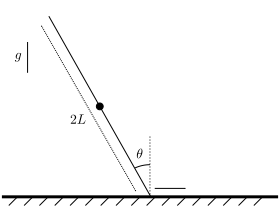
\includegraphics{rod_slip.pdf}
\end{center}


\end{document}
